% 第四章 霍普夫子 动力学调控
\chapter{霍普夫子 动力学调控}

自旋波作为一种非接触式调控手段，在驱动二维磁性拓扑结构方面已有较多研究\cite{ding2015motion,huang2023transient,shen2018skyrmionium}。对于三维霍普夫子，现有工作主要从理论解析角度探讨其与磁振子的耦合机制\cite{saji2023magnonic}，或分析反铁磁背景下的自旋波散射过程\cite{zhang2023magnon}。针对铁磁体系中自旋波对霍普夫子的直接驱动机制，目前尚缺乏系统的微磁学数值论证。本章以此为切入点，研究阻挫交换铁磁体系中霍普夫子在自旋波激励下的动力学响应与调控规律。


与电流驱动相比，自旋波以非接触方式传递角动量，焦耳热损耗显著降低，能量利用效率更高。本章以第三章确定的阻挫交换铁磁体系为仿真平台，系统扫描传播方向与振荡方向的不同组合对 霍普夫子 运动行为的影响。

\section{仿真模型与自旋波激励源}

\subsection{模型设置与激励方案}
材料参数和网格规格均继承自第三章的阻挫交换铁磁体系（\cref{tab:frustrated-params}），模拟区域为 $100 \times 100 \times 100$ 格点、间距 $\SI{0.5}{nm}$。边界条件方面，本章与第三章的周期性设置不同，转而采用吸收边界方案，在六面各设置 5 格厚度（约 $\SI{2.5}{nm}$）的高阻尼层（$\alpha = 100$），其作用是衰减边界处的自旋波反射，近似地模拟开放边界环境。体区阻尼保持为 $\alpha = 0.001$。

激励源设定为厚度 $\SI{0.5}{nm}$ 的薄片层，施加正弦振荡外磁场 $\mathbf{B}_{\text{ext}} = B_0 \sin(2\pi f t) \, \hat{n}$；默认频率与振幅分别取 $f = \SI{440}{GHz}$ 和 $B_0 = \SI{1}{T}$。磁化初始构型采用第三章各向异性扫描中 $K_{u1} = \SI{10e3}{J/m^3}$ 所对应的居中弛豫态。

上述参数中，网格间距 $\SI{0.5}{nm}$ 与模型尺寸 $100 \times 100 \times 100$ 沿用第三章（\cref{tab:frustrated-params}），可分辨平衡管径 $r_{\text{eq}} = \SI{2.16}{nm}$；吸收边界 5 格高阻尼层是 Mumax3 模拟开放边界的常规做法\cite{vansteenkiste2014design}；激励幅度 $B_0 = \SI{1}{T}$ 取自此前自旋波驱动磁性拓扑结构的常用强驱动量级\cite{ding2015motion,sallermann2023stability}。本研究所用参数足以稳定再现霍普夫子稳态构型与频率响应特征，更细网格、更厚吸收层下的系统性敏感性扫描留待后续工作。

鉴于 霍普夫子 在 $xy$ 平面内具有旋转对称性，只需选取 4 种具有代表性的方向组合即可覆盖主要的物理场景，具体编号及物理含义列于\cref{tab:sw-combos}。为便于后文表述，本文统一采用 src$A$\_vib$B$ 的简记方式命名每个驱动组合。其中 src$A$（$A \in \{X, Y, Z\}$）标识激励源所在平面，对应源平面位于 $A = -\SI{10}{nm}$ 处；vib$B$（$B \in \{X, Z\}$）标识外场振荡方向，对应 $\hat{n} = \hat{B}$。例如 srcX\_vibX 表示源平面位于 $x = -\SI{10}{nm}$、振荡沿 $\hat{x}$ 的组合。

\begin{table}[htbp]
  \centering
  \caption{自旋波驱动实验的 4 种组合（srcA 表示激励源所在平面，vibB 表示外场振荡方向）。}
  \label{tab:sw-combos}
  \begin{tabular}{cccl}
    \toprule
    组合 & 源位置 & 振荡方向 & 物理含义 \\
    \midrule
    srcX\_vibX & $x = -\SI{10}{nm}$ & $\hat{x}$ & 面内传播，面内振荡 \\
    srcX\_vibZ & $x = -\SI{10}{nm}$ & $\hat{z}$ & 面内传播，面外振荡 \\
    srcZ\_vibX & $z = -\SI{10}{nm}$ & $\hat{x}$ & 轴向传播，面内振荡 \\
    srcZ\_vibZ & $z = -\SI{10}{nm}$ & $\hat{z}$ & 轴向传播，轴向振荡 \\
    \bottomrule
  \end{tabular}
\end{table}

\subsection{平面源与点源的对比}
以上各组仿真全部基于平面波激励（$\SI{0.5}{nm}$ 厚薄片层，$B_0 = \SI{1}{T}$）。为评估激励源几何形态对驱动规律的影响，本节补充点源激励对照实验。点源的实现方式是将体积为 $\SI{0.5}{nm}^3$ 的单个网格单元单独定义为激励区域，并仅在该单元上施加正弦振荡外场 $\mathbf{B}_{\text{ext}}(t) = B_0 \sin(2\pi f t)\, \hat{n}$，模拟区域内其余位置不施加外场。

为保证与平面源结果的可比性，点源中心严格对齐于平面源所在位置：srcX 点源置于网格指标 $(i_x, i_y, i_z) = (30, 50, 50)$，对应物理坐标 $(-10, 0, 0)\,\si{nm}$；srcZ 点源置于 $(50, 50, 30)$，对应 $(0, 0, -10)\,\si{nm}$，二者均与\cref{tab:sw-combos}所列平面源位置一致。激励幅度由平面源的 $B_0 = \SI{1}{T}$ 提升至 $B_0 = \SI{500}{T}$。按平面源体积 $\SI{1250}{nm^3}$ 对点源 $\SI{0.125}{nm^3}$ 的体积比 $\sim 10^4$ 估算，能量通量等效需放大约 $\sqrt{10^4} = 100$ 倍，本文取 500 倍以补偿点源辐射的方向性损失；该值仅为受控对照的等效驱动强度，非实验可行场强。材料参数、吸收边界设置以及初始磁化构型与平面源完全一致。在 srcX 与 srcZ 两个传播方向上分别实施 $\SIrange{100}{1000}{GHz}$ 的 10 点频率扫描。

\begin{figure}[H]
  \centering
  
\includegraphics[width=0.8\textwidth]{figures/fig4-12_point_source_freq_response.png}
  \caption{点源驱动下的频率响应谱。(a) srcX（面内传播）: $|\Delta r|(f)$; (b) srcZ（轴向传播）: $|\Delta r|(f)$。绿色、橙色柱分别代表 $+z$、$-z$ 方向。}
  \label{fig:point-source-freq}
\end{figure}

\cref{fig:point-source-freq} 的数据反映出点源与平面源驱动在定量特征上的差异。一方面共振频率发生偏移，点源条件下的响应峰值频率相较于平面源出现红移；另一方面主导方向特征得以保持。上述对照实验表明，霍普夫子在自旋波响应中的极化选择性与运动方向互补特征主要由其固有拓扑属性决定，对激励源的几何形态不敏感。后文的系统性仿真即以平面源为主进行。

\section{自旋波驱动性质}
\label{subsec:freq-sweep}

\subsection{方向选择性}
全部 5 组仿真的定量结果汇总在\cref{tab:drive-selection}与\cref{fig:direction-selectivity}中。以 $\SI{0.5}{ns}$ 时刻霍普夫子质心的净位移 $|\Delta r|$ 作为判据，驱动组合被清晰地分为有效与无效两类。一方面，srcX\_vibX、srcY\_vibX 与 srcZ\_vibX 三组构成有效驱动组（$|\Delta r| > \SI{1}{nm}$），均引发了可观测的霍普夫子位移，其中最大的是 srcZ\_vibX（$|\Delta r| = \SI{6.71}{nm}$），srcX\_vibX（$\SI{2.36}{nm}$）与 srcY\_vibX（$\SI{2.31}{nm}$）次之。另一方面，srcX\_vibZ 与 srcZ\_vibZ 两组构成无效驱动组（$|\Delta r| < \SI{0.01}{nm}$），霍普夫子基本静止，位移停留在噪声量级（$< \SI{0.006}{nm}$），能量变化也仅 $\sim\SI{3e-21}{J}$，不足有效组合的 $1\%$。上述定量数据反映出驱动过程具有极化依赖特性。面内振荡（$\hat{x}$）能够有效激发霍普夫子发生平动，而面外振荡（$\hat{z}$）无法产生有效位移。该现象的物理机制在于面外振荡维持了拓扑结构的轴对称性，限制了向平动模式的角动量耦合，面内振荡则打破了该对称性并促成了能量转换。此外 srcX\_vibX 与 srcY\_vibX 组合下相近的位移量印证了面内传播的各向同性，与霍普夫子在 $xy$ 平面内的旋转对称特征相自洽。

\begin{table}[htbp]
  \centering
  \caption{5 种自旋波组合的 霍普夫子 驱动结果（$f = \SI{440}{GHz}$, $B_0 = \SI{1}{T}$, $t = \SI{0.5}{ns}$）。}
  \label{tab:drive-selection}
  \begin{tabular}{ccrrrc}
    \toprule
    传播方向 & 振荡方向 & $\Delta z$ (nm) & $|\Delta r|$ (nm) & $\Delta E$ (J) & 判定 \\
    \midrule
    面内 $\hat{x}$ & 面内 $\hat{x}$ & $+2.355$ & $2.358$ & $4.15 \times 10^{-19}$ & 有效 \\
    面内 $\hat{x}$ & 面外 $\hat{z}$ & $+0.005$ & $0.005$ & $3.38 \times 10^{-21}$ & 无效 \\
    面内 $\hat{y}$ & 面内 $\hat{x}$ & $+2.307$ & $2.310$ & $4.20 \times 10^{-19}$ & 有效 \\
    轴向 $\hat{z}$ & 面内 $\hat{x}$ & $-6.706$ & $6.706$ & $2.51 \times 10^{-19}$ & 有效 \\
    轴向 $\hat{z}$ & 轴向 $\hat{z}$ & $-0.001$ & $0.001$ & $3.24 \times 10^{-21}$ & 无效 \\
    \bottomrule
  \end{tabular}
\end{table}

\begin{figure}[H]
  \centering
  
\includegraphics[width=0.85\textwidth]{figures/fig4-1_direction_selectivity.png}
  \caption{5 种驱动组合下 霍普夫子 质心坐标的时间演化。(a) $\Delta x(t)$; (b) $\Delta y(t)$; (c) $\Delta z(t)$; (d) 总位移 $|\Delta\mathbf{r}|(t)$。}
  \label{fig:direction-selectivity}
\end{figure}

需要指出的是，三个有效组合在运动方向上展现出系统性的分化特征。srcX\_vibX 与 srcY\_vibX 均将 霍普夫子 推向 $+z$，即垂直于自旋波传播方向；srcZ\_vibX 产生的迁移则沿 $-z$ 进行，与传播方向平行。这种 $+z$ 与 $-z$ 的方向互补性，为后文设计双向轴向控制方案奠定了物理基础。

确认面内振荡（vibX）为有效的驱动模式之后，本研究分别对面内传播（srcX）与轴向传播（srcZ）实施频率扫描，以揭示 霍普夫子 运动对激励频率的依赖规律。

\subsection{面内传播 srcX 的频率响应}

固定 srcX\_vibX 组合与 $B_0 = \SI{1}{T}$ 的驱动幅度，本文在 $\SIrange{100}{1000}{GHz}$ 区间以 $\SI{100}{GHz}$ 步长扫描。各频率下 霍普夫子 的位移与速度的时间关系如\cref{fig:srcX-displacement}。

\begin{figure}[H]
  \centering
  
\includegraphics[width=0.85\textwidth]{figures/fig4-3_srcX_displacement.png}
  \caption{srcX（面内传播）驱动下 霍普夫子 位移与瞬时速度的时间演化。(a) 总位移 $|\Delta r|(t)$; (b) $\Delta x(t)$; (c) $\Delta z(t)$; (d) 瞬时速度 $|v|(t)$。}
  \label{fig:srcX-displacement}
\end{figure}

仿真数据呈现出频率选择性特征。低频区 $\SIrange{100}{200}{GHz}$与高频区 $\SI{1000}{GHz}$共同划定了有效驱动窗口。$\SIrange{400}{600}{GHz}$ 频段 霍普夫子 近乎完全静止，可判定为死区；$\SIrange{700}{900}{GHz}$ 段的响应则处于过渡状态。本研究注意到，无论频率如何变化，霍普夫子 始终沿 $+z$ 方向迁移，运动方向并不随频率发生翻转。

\subsection{轴向传播 srcZ 的频率响应}

转向 srcZ 驱动时，频率扫描范围拓宽至 $\SIrange{25}{1500}{GHz}$，累计覆盖 20 个采样点。从中选取 8 个代表性频率，其位移与瞬时速度的时间关系如\cref{fig:srcZ-trajectory}。

\begin{figure}[H]
  \centering
  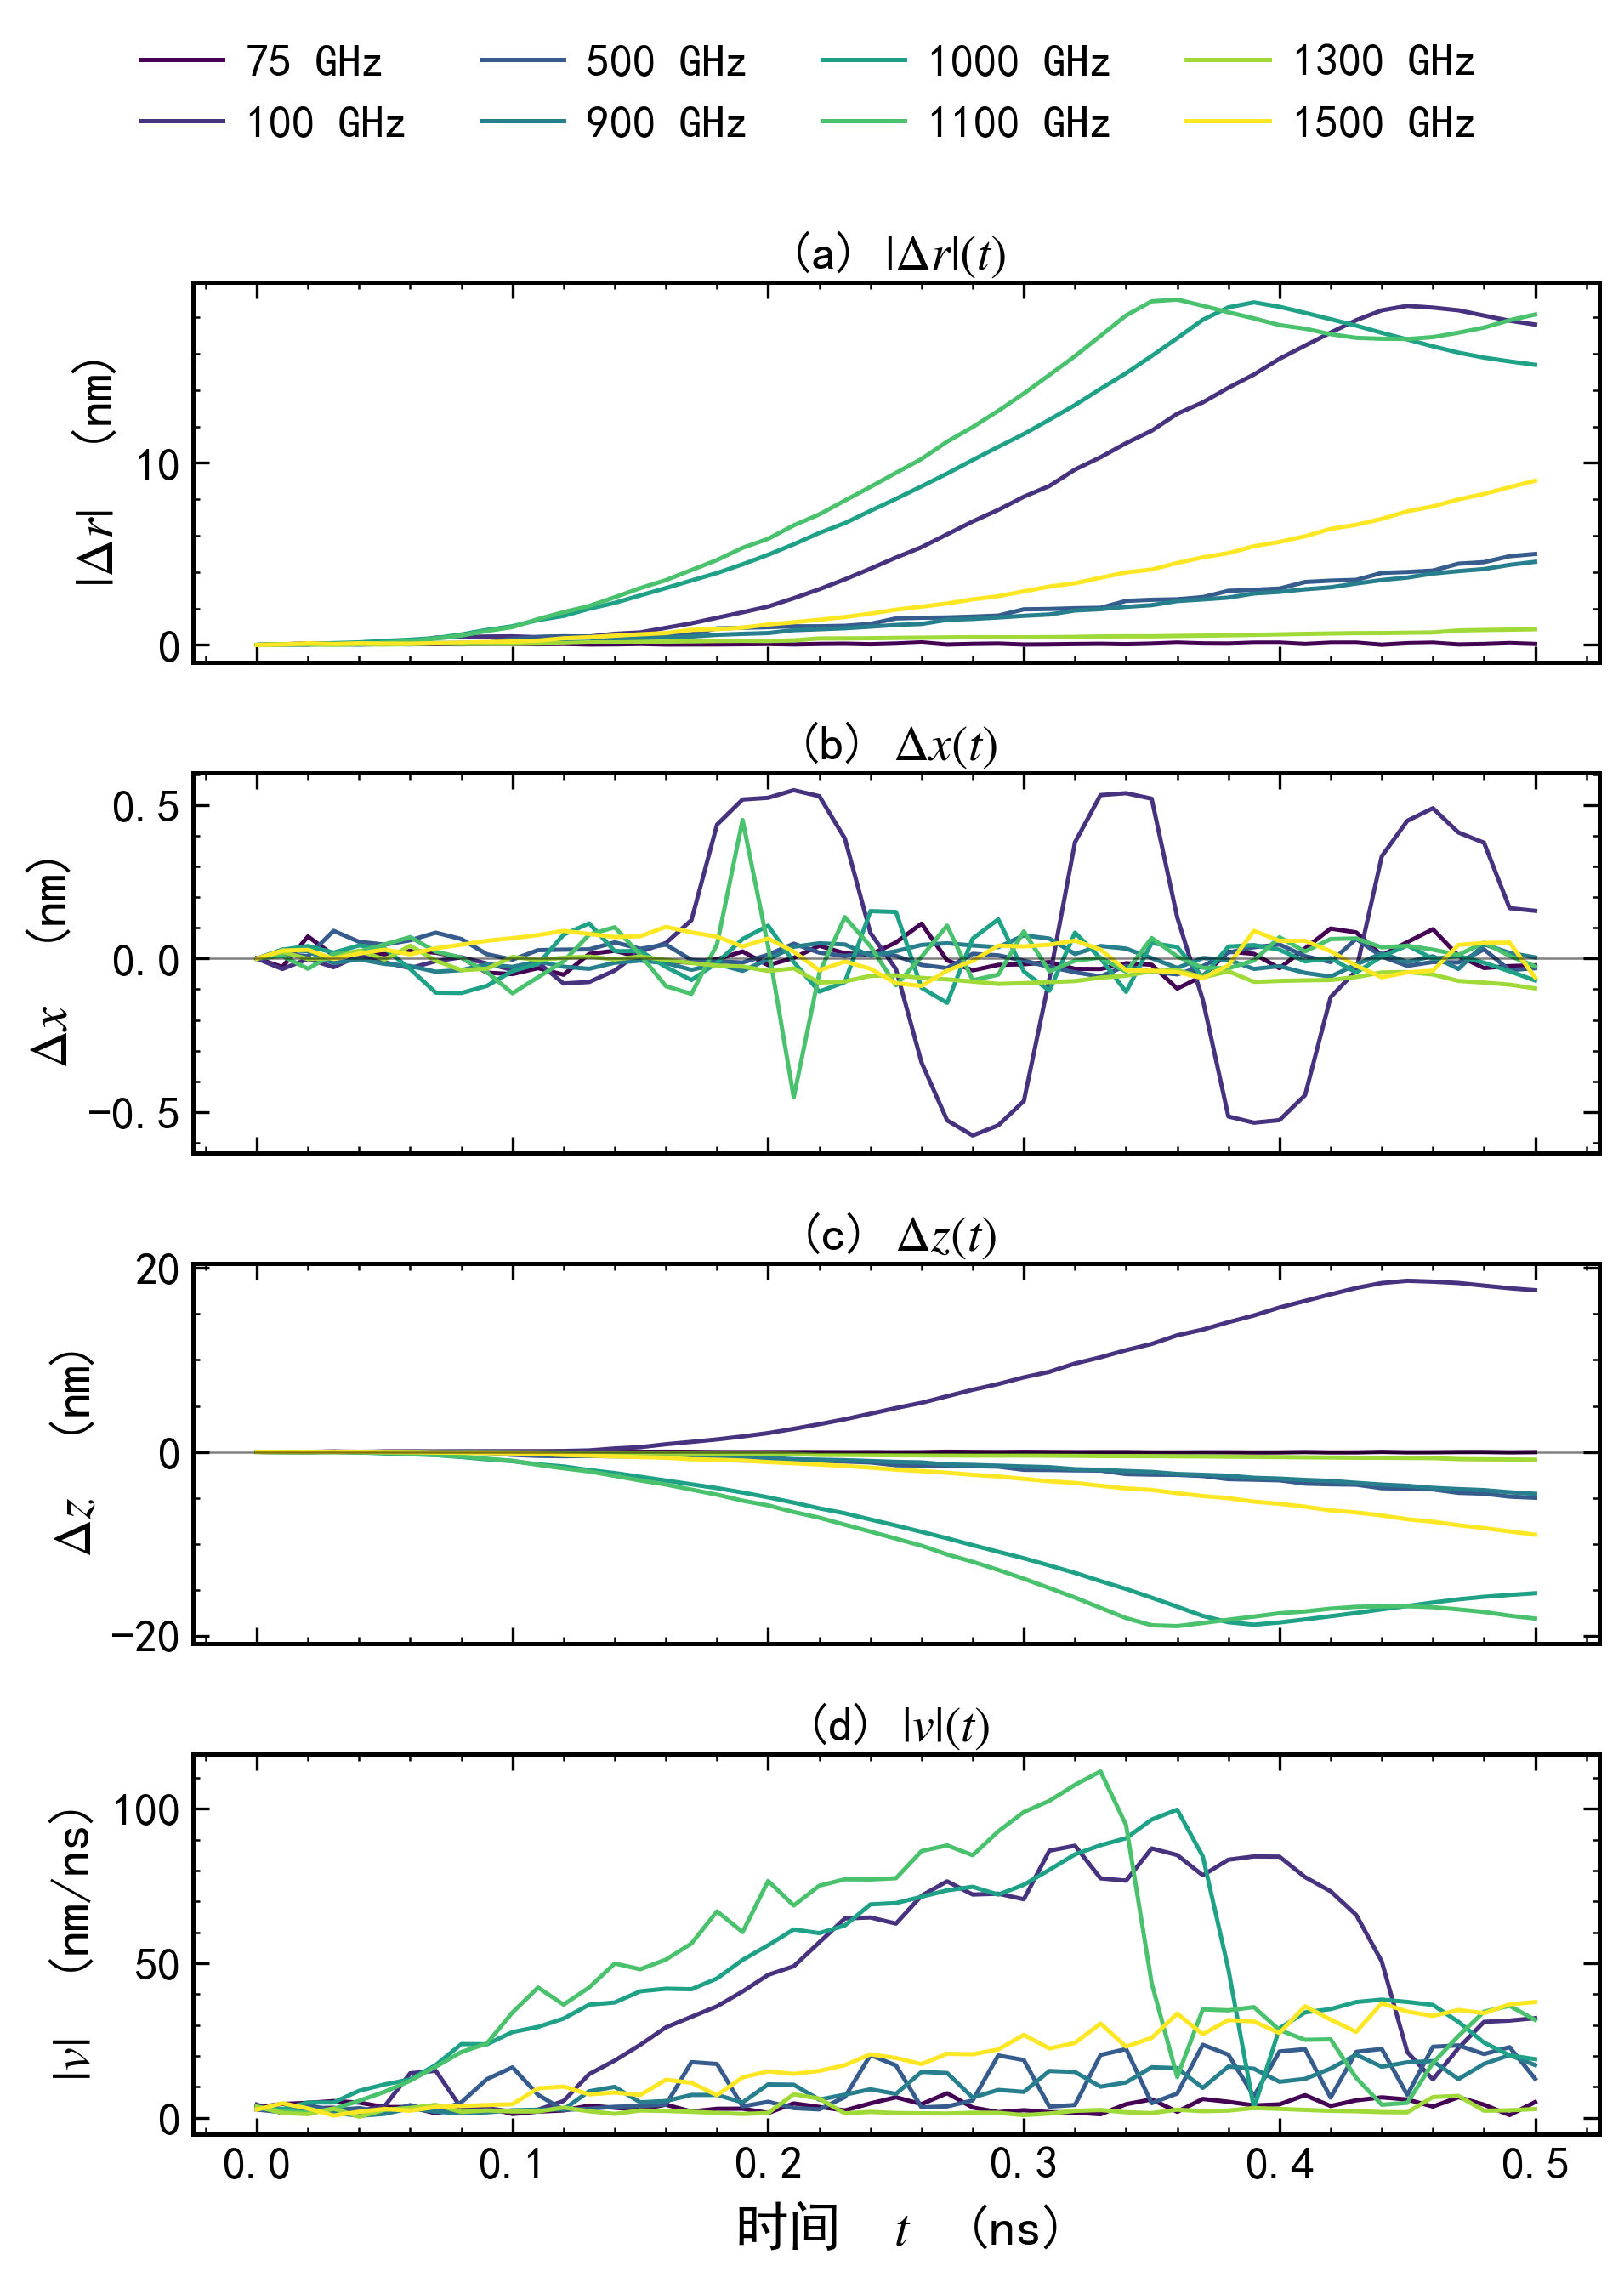
\includegraphics[width=0.85\textwidth]{figures/fig4-5_srcZ_trajectory.png}
  \caption{srcZ（轴向传播）驱动下 8 个代表频率点 霍普夫子 位移与瞬时速度的时间演化。(a) 总位移 $|\Delta r|(t)$; (b) $\Delta x(t)$; (c) $\Delta z(t)$; (d) 瞬时速度 $|v|(t)$。}
  \label{fig:srcZ-trajectory}
\end{figure}

srcZ 的频谱与 srcX 呈现截然不同，如下三个维度。（1）方向集中于单一频率，在全部 20 个采样点中，仅 $\SI{100}{GHz}$ 引导 霍普夫子 朝 $+z$（即朝向激励源）运动，其余 19 个频率无一例外地驱动 $-z$（远离源）方向的迁移。（2）共振谱呈多峰结构，$\SI{1100}{GHz}$ 处出现最强共振，$\SI{100}{GHz}$和 $\SI{1000}{GHz}$分列次强；死区散布于 $\SI{75}{GHz}$、$\SI{150}{GHz}$、$\SI{600}{GHz}$ 及 $\SI{1300}{GHz}$ 等处。（3）运动模式随响应强度分化，强响应频率点的 霍普夫子 以匀速模式运动，弱响应点则表现出加速的时间演化特征。

两种传播方向在响应特性上的差别，其根源在于各自与 霍普夫子 内模的耦合通道不同。面内传播（srcX）优先激发面内平动模式，驱动 霍普夫子 沿 $+z$ 方向迁移，即垂直于自旋波传播方向；轴向传播（srcZ）则直接作用于轴向平动通道，霍普夫子 顺势沿 $-z$ 方向运动。耦合通道的差异同时决定了二者的共振频率分布呈现出互不重叠的特征。值得注意的是，srcZ 在 $\SI{100}{GHz}$ 的反向位移还伴随着体系向驱动场的净能量回流，说明该频率点存在与其余频率不同的相干耦合路径。

\subsection{驱动幅度响应}
\label{subsec:amplitude-scaling}
在组合为 srcX\_vibX、频率固定在 $f = \SI{440}{GHz}$ 的条件下，本文对 $B_0 = \SIrange{0.05}{2.0}{T}$ 范围内的 6 个幅度实施仿真，以寻找自旋波驱动的有效幅度区间。

\begin{figure}[H]
  \centering
  
\includegraphics[width=0.85\textwidth]{figures/fig4-8_amplitude_trajectory.png}
  \caption{不同驱动幅度下 霍普夫子 的位移时间演化。(a) 总位移 $|\Delta r|(t)$; (b) $\Delta z(t)$。}
  \label{fig:amplitude-trajectory}
\end{figure}

\cref{fig:amplitude-trajectory}表明，在 $B_0 \geq \SI{0.5}{T}$ 区段中 霍普夫子 被自旋波持续推动，位移随幅度的增大而增大；而在 $B_0 \leq \SI{0.1}{T}$ 的弱驱动段，位移迅速衰减至噪声水平（$|\Delta r| < \SI{0.1}{nm}$），体系失去有效响应。本节仅针对该幅度窗口作定性界定，$B_0^\alpha$ 标度律的精确确定需更密集的幅度扫描与更长的仿真时长，留待后续工作。

\section{自旋波驱动应用}
\label{subsec:bidirectional-control}

前文数据已经清楚地表明，srcX 驱动 $+z$ 运动（垂直于传播方向），srcZ 驱动 $-z$ 运动（沿传播方向）。这意味着仅需在两种传播方向之间切换，即可实现 霍普夫子 在 $z$ 轴上的双向可控迁移。此外，srcZ 传播模式在频率域上具有方向反转特征，这提供了一种基于单一波源的调控方案，通过切换激发频率即可实现霍普夫子运动方向的反转。

\begin{figure}[H]
  \centering
  
\includegraphics[width=0.9\textwidth]{figures/fig4-10_multisource_baseline.png}
  \caption{三种单源基线的 霍普夫子 轨迹对比（$f = \SI{200}{GHz}$, vibX 表示外场沿 $\hat{x}$ 振荡）。(a) $\Delta x(t)$; (b) $\Delta y(t)$; (c) $\Delta z(t)$。}
  \label{fig:multisource-baseline}
\end{figure}

srcX 与 srcZ 两类单源基线的运动轨迹在\cref{fig:multisource-baseline}中进行了直观的对比，方向互补性一目了然。

为对频率切换方案进行直接验证，本文设计了两阶段的分时序仿真实验。Phase~1 阶段（$0$--$\SI{0.50}{ns}$）施加 srcZ@$\SI{100}{GHz}$，驱使 霍普夫子 向 $+z$ 迁移；Phase~2 阶段（$\SI{0.50}{}$--$\SI{0.80}{ns}$）将频率切换至 srcZ@$\SI{1100}{GHz}$，预期驱动 $-z$ 方向的反向运动。

仿真结果（\cref{fig:freq-switch-z}）显示，Phase~1 内 霍普夫子 沿 $+z$ 稳定迁移，累计位移攀升至峰值 $\SI{+18.6}{nm}$。频率在 Phase~2 起始时刻切换为 $\SI{1100}{GHz}$ 后，霍普夫子 立即翻转至 $-z$ 方向运动，仅经 $\SI{0.30}{ns}$ 便从峰值 $+\SI{18.6}{nm}$ 回落至 $+\SI{4.0}{nm}$。位移曲线整体呈现先攀升后回落的非单调特征。从仿真结果来看，这种先积累后释放的演化轨迹在波形上与生物神经元膜电位的充放电过程具有形态相似性（第六章将对此展开讨论）。

上述实验直接证实了单一 srcZ 激励源通过频率切换即可实现 霍普夫子 运动方向的完全反转。Phase~2 中 $-z$ 方向的运动速度显著高于 Phase~1 中 $+z$ 方向的速度，反映出 $\SI{1100}{GHz}$ 与 $\SI{100}{GHz}$ 两个频率在耦合强度上的明显差异。

\begin{figure}[H]
  \centering
  
\includegraphics[width=0.9\textwidth]{figures/fig4-11_freq_switch_z_control.png}
  \caption{频率切换下双向 $z$ 轴控制的验证结果。(a) $z$ 方向位移 $\Delta z(t)$; (b) $z$ 方向速度 $v_z(t)$。绿色区对应 srcZ@$\SI{100}{GHz}$（$0$--$\SI{0.50}{ns}$，$+z$），蓝色区对应 srcZ@$\SI{1100}{GHz}$（$\SI{0.50}{}$--$\SI{0.80}{ns}$，$-z$）。}
  \label{fig:freq-switch-z}
\end{figure}

本章利用微磁学仿真系统考察了自旋波驱动下霍普夫子的动力学行为。结果显示驱动过程具有严格的极化依赖性，面内振荡是激发有效平动的必要条件。在频率响应方面，面内传播与轴向传播模式表现出不同的共振峰，前者驱动霍普夫子垂直于传播方向运动，后者则促使其平行于传播方向迁移。基于这两种模式的方向互补性及特定频率下的方向反转现象，验证了依靠单频切换实现 $z$ 轴双向控制的可行性。此外对照实验确认，上述拓扑响应特征主要由霍普夫子的固有属性决定，对自旋波激励几何具有较强的抗干扰能力。
